\documentclass[a4paper,12pt]{ltjsarticle}

% LuaTeX-ja の設定
\usepackage{luatexja}
\usepackage{luatexja-fontspec}
\usepackage[margin=2.5cm]{geometry}

% 数学パッケージ
\usepackage{amsmath,amssymb,amsthm}
\usepackage{mathtools}

% 図式とグラフィックス
\usepackage{tikz}
\usetikzlibrary{arrows,positioning,matrix,calc,decorations.pathreplacing}

% その他のパッケージ
\usepackage{xcolor}
\usepackage{hyperref}
\usepackage{enumitem}
\usepackage{tcolorbox}

% 定理環境の設定
\theoremstyle{definition}
\newtheorem{definition}{定義}[section]
\newtheorem{theorem}[definition]{定理}
\newtheorem{lemma}[definition]{補題}
\newtheorem{proposition}[definition]{命題}
\newtheorem{corollary}[definition]{系}
\newtheorem{example}[definition]{例}
\newtheorem{remark}[definition]{注意}

% カスタムボックス
\tcbuselibrary{theorems}
\newtcolorbox{axiombox}{
  colback=blue!5!white,
  colframe=blue!75!black,
  title=公理
}

\newtcolorbox{leanbox}{
  colback=green!5!white,
  colframe=green!50!black,
  title=Lean実装
}

% タイトル情報
\title{構造塔理論による\\離散時間マルチンゲール理論の形式化}
\author{%
  \textbf{著者:}\\[0.5em]
  Codex (OpenAI) --- Leanコード生成\\
  Claude Code (Anthropic) --- \TeX{}ドキュメント生成\\[1em]
  \textbf{プロジェクト:} Structure Tower Project
}
\date{\today}

\begin{document}

\maketitle

\begin{abstract}
本文書は、離散時間マルチンゲール理論をBourbaki流の集合論的アプローチで形式化したLeanコードについての数学的解説である。フィルトレーション、停止時刻、マルチンゲール、任意停止定理、Doob分解などの基本概念を、構造塔(structure tower)という統一的枠組みで再構成する。各概念の定義、主要な定理、およびそれらの相互関係を詳述し、測度論的な詳細を公理化することで、理論の本質的な構造を明らかにする。

\textbf{注:} 本文書のLeanコードはCodex (OpenAI)により生成され、本\TeX{}ドキュメントはClaude Code (Anthropic)により生成された。
\end{abstract}

\tableofcontents
\clearpage

% ========================================
\section{序論}

確率論におけるマルチンゲール理論は、確率過程の解析において中心的な役割を果たす。本文書では、この理論を離散時間設定において形式化し、Lean証明支援系での実装について解説する。

我々のアプローチの特徴は、\textbf{構造塔(structure tower)}という抽象的枠組みを用いて、測度論的な詳細を公理化し、理論の本質的な構造を抽出する点にある。これはBourbakiの精神に則った、集合論的・構造主義的なアプローチである。

\subsection{構造塔とは}

構造塔は、層(layer)により階層化された対象の族を扱うための抽象的枠組みである。時間パラメータ$n \in \mathbb{N}$に対して、各時刻における「情報」の集まりを層として表現する。

確率論の文脈では:
\begin{itemize}
  \item \textbf{層} $\to$ 時刻$n$における可測事象の族(フィルトレーション)
  \item \textbf{層の単調性} $\to$ 情報の増大
  \item \textbf{最小層} $\to$ 事象が初めて観測される時刻
\end{itemize}

\subsection{本文書の構成}

\begin{enumerate}
  \item \textbf{Level 1}: 離散フィルトレーションと停止時刻の基礎理論
  \item \textbf{Level 2.1}: マルチンゲール、サブマルチンゲール、スーパーマルチンゲールの定義
  \item \textbf{Level 2.2}: 停止された過程と任意停止定理
  \item \textbf{Level 2.3}: Doob分解理論
  \item \textbf{Level 2.5}: 停止時刻の代数的操作
\end{enumerate}

% ========================================
\section{Level 1: 離散フィルトレーションと停止時刻}

\subsection{離散フィルトレーション}

\begin{definition}[離散フィルトレーション]
標本空間$\Omega$上の\textbf{離散フィルトレーション}とは、以下のデータからなる:
\begin{enumerate}
  \item 各時刻$n \in \mathbb{N}$に対する事象の族$\sigma_n \subseteq \mathcal{P}(\Omega)$
  \item 単調性: $m \leq n \Rightarrow \sigma_m \subseteq \sigma_n$
  \item 被覆性: 任意の事象$E \subseteq \Omega$に対して、$E \in \sigma_n$となる$n$が存在
\end{enumerate}
\end{definition}

\begin{leanbox}
\begin{verbatim}
structure DiscreteFiltration (Ω : Type u) where
  sigma : ℕ → Set (Set Ω)
  mono : Monotone sigma
  covering : ∀ E : Set Ω, ∃ n : ℕ, E ∈ sigma n
\end{verbatim}
\end{leanbox}

\begin{remark}
通常の確率論では$\sigma_n$は$\sigma$-代数であるが、ここでは集合の族として扱う。測度論的な詳細(可算加法性など)は公理化により回避される。
\end{remark}

\subsubsection{構造塔への埋め込み}

フィルトレーション$\mathcal{F} = (\sigma_n)_{n \in \mathbb{N}}$は、自然に構造塔を定める:

\begin{center}
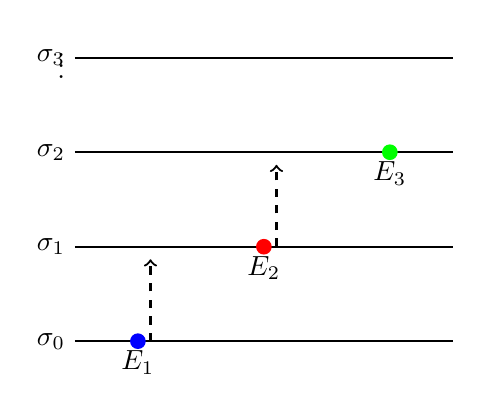
\begin{tikzpicture}[scale=0.8]
  % 層の描画
  \foreach \n in {0,1,2,3} {
    \draw[thick] (0,\n*1.5) -- (6,\n*1.5);
    \node[left] at (0,\n*1.5) {$\sigma_{\n}$};
  }
  \node[left] at (0,4.5) {$\vdots$};

  % 事象の配置
  \node[circle,fill=blue,inner sep=2pt] at (1,0) {};
  \node[below] at (1,0) {$E_1$};

  \node[circle,fill=red,inner sep=2pt] at (3,1.5) {};
  \node[below] at (3,1.5) {$E_2$};

  \node[circle,fill=green,inner sep=2pt] at (5,3) {};
  \node[below] at (5,3) {$E_3$};

  % 単調性の矢印
  \draw[->,thick,dashed] (1.2,0) -- (1.2,1.3);
  \draw[->,thick,dashed] (3.2,1.5) -- (3.2,2.8);
\end{tikzpicture}
\end{center}

各事象$E$は、それが初めて観測される層$\sigma_n$に配置される。これが\textbf{最小層}$\mathrm{minLayer}(E)$である。

\subsection{停止時刻}

\begin{definition}[停止時刻]
フィルトレーション$\mathcal{F}$に適合する\textbf{停止時刻}$\tau$とは、写像$\tau : \Omega \to \mathbb{N}$であって、各$n \in \mathbb{N}$に対して
\[
  \{\omega \in \Omega \mid \tau(\omega) \leq n\} \in \sigma_n
\]
を満たすものである。
\end{definition}

\begin{leanbox}
\begin{verbatim}
structure StoppingTime (F : DiscreteFiltration Ω) where
  value : Ω → ℕ
  adapted : ∀ n : ℕ, {ω : Ω | value ω ≤ n} ∈ F.sigma n
\end{verbatim}
\end{leanbox}

\begin{remark}[停止時刻の直観]
停止時刻は「未来の情報を使わずに決定できる時刻」を表す。時刻$n$において、$\tau \leq n$という事象が判定可能でなければならない。
\end{remark}

\subsubsection{停止時刻の構造塔表現}

停止時刻$\tau$もまた構造塔を定める:

\begin{center}
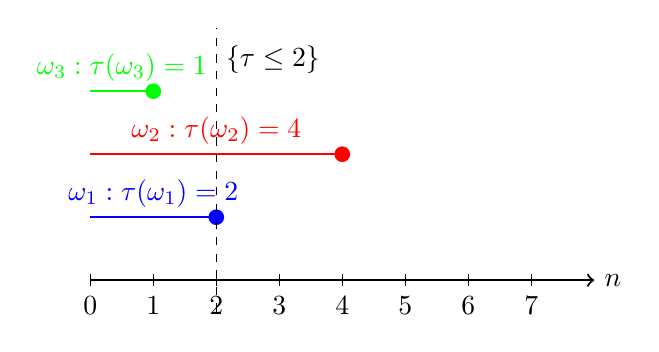
\begin{tikzpicture}[scale=0.8]
  % 時間軸
  \draw[->,thick] (0,0) -- (8,0) node[right] {$n$};
  \foreach \n in {0,1,2,3,4,5,6,7} {
    \draw (\n,0.1) -- (\n,-0.1) node[below] {$\n$};
  }

  % 軌道の例
  \draw[thick,blue] (0,1) -- (2,1) node[circle,fill=blue,inner sep=2pt] {};
  \node[above,blue] at (1,1) {$\omega_1: \tau(\omega_1) = 2$};

  \draw[thick,red] (0,2) -- (4,2) node[circle,fill=red,inner sep=2pt] {};
  \node[above,red] at (2,2) {$\omega_2: \tau(\omega_2) = 4$};

  \draw[thick,green] (0,3) -- (1,3) node[circle,fill=green,inner sep=2pt] {};
  \node[above,green] at (0.5,3) {$\omega_3: \tau(\omega_3) = 1$};

  % 事象の表示
  \draw[dashed] (2,-0.5) -- (2,4);
  \node[right] at (2,3.5) {$\{\tau \leq 2\}$};
\end{tikzpicture}
\end{center}

各標本点$\omega$は、時刻$\tau(\omega)$で「停止」する。

\subsection{自明なフィルトレーション}

\begin{definition}[自明なフィルトレーション]
\textbf{自明なフィルトレーション}は、すべての事象が時刻$0$から可視である:
\[
  \sigma_n = \mathcal{P}(\Omega) \quad \forall n \in \mathbb{N}
\]
\end{definition}

これは「情報が増大しない」極端な例である。

% ========================================
\section{Level 1 拡張: フィルトレーションと確率過程}

\subsection{確率過程の適合性}

\begin{definition}[適合確率過程]
値空間$\beta$を持つ確率過程$X = (X_n)_{n \in \mathbb{N}}$が、フィルトレーション$\mathcal{F}$に\textbf{適合}するとは、各時刻$n$と各$b \in \beta$に対して
\[
  \{w \in \Omega \mid X_n(\omega) = b\} \in \sigma_n
\]
が成り立つことである。
\end{definition}

\begin{leanbox}
\begin{verbatim}
structure StochasticProcess
    (F : DiscreteFiltration Ω) (β : Type v) [DecidableEq β] where
  value : ℕ → Ω → β
  adapted : ∀ n b, {ω : Ω | value n ω = b} ∈ F.sigma n
\end{verbatim}
\end{leanbox}

\subsection{条件付き期待値の公理化}

\begin{definition}[条件付き期待値構造]
フィルトレーション$\mathcal{F}$上の\textbf{条件付き期待値構造}とは、作用素の族
\[
  \mathbb{E}[\cdot \mid \mathcal{F}_n] : (\Omega \to \mathbb{R}) \to (\Omega \to \mathbb{R})
\]
であって、\textbf{塔性質(tower property)}:
\[
  m \leq n \Rightarrow \mathbb{E}[\mathbb{E}[X \mid \mathcal{F}_n] \mid \mathcal{F}_m] = \mathbb{E}[X \mid \mathcal{F}_m]
\]
を満たすものである。
\end{definition}

\begin{leanbox}
\begin{verbatim}
structure ConditionalExpectationStructure
    (F : DiscreteFiltration Ω) where
  cond : ℕ → (Ω → ℝ) → Ω → ℝ
  tower : ∀ m n (X : Ω → ℝ), m ≤ n →
      cond m (cond n X) = cond m X
\end{verbatim}
\end{leanbox}

\begin{center}
\begin{tikzpicture}[node distance=2cm]
  \node (X) {$X$};
  \node (En) [below left of=X] {$\mathbb{E}[X \mid \mathcal{F}_n]$};
  \node (Em) [below of=En] {$\mathbb{E}[X \mid \mathcal{F}_m]$};

  \draw[->,thick] (X) -- (En) node[midway,above left] {条件付き期待値};
  \draw[->,thick] (En) -- (Em) node[midway,left] {さらに条件付け};
  \draw[->,thick,dashed] (X) -- (Em) node[midway,right] {直接};

  \node[right of=Em,xshift=1cm] {$m \leq n$};
\end{tikzpicture}
\end{center}

塔性質は「情報を忘れる操作は冪等的」という直観を表す。

% ========================================
\section{Level 2.1: マルチンゲール理論}

\subsection{マルチンゲールの定義}

\begin{definition}[マルチンゲール]
実数値確率過程$X = (X_n)_{n \in \mathbb{N}}$が\textbf{マルチンゲール}であるとは、以下を満たすことである:
\begin{enumerate}
  \item 適合性: 各$n, r$に対して$\{\omega \mid X_n(\omega) \leq r\} \in \sigma_n$
  \item マルチンゲール条件: $m \leq n \Rightarrow \mathbb{E}[X_n \mid \mathcal{F}_m] = X_m$
\end{enumerate}
\end{definition}

\begin{leanbox}
\begin{verbatim}
structure IsMartingale
    (F : DiscreteFiltration Ω)
    (C : ConditionalExpectationStructure F)
    (X : ℕ → RandomVariable Ω) : Prop where
  adapted : ∀ n r, {ω : Ω | X n ω ≤ r} ∈ F.sigma n
  martingale_condition : ∀ {m n}, m ≤ n → C.cond m (X n) = X m
\end{verbatim}
\end{leanbox}

\begin{remark}[マルチンゲールの直観]
マルチンゲール条件$\mathbb{E}[X_n \mid \mathcal{F}_m] = X_m$は、「過去の情報に基づく未来の予測値は、現在の値に等しい」ことを意味する。これは「公平なゲーム」の数学的モデルである。
\end{remark}

\subsection{サブマルチンゲールとスーパーマルチンゲール}

\begin{definition}[サブマルチンゲール]
確率過程$X$が\textbf{サブマルチンゲール}であるとは、
\[
  m \leq n \Rightarrow X_m \leq \mathbb{E}[X_n \mid \mathcal{F}_m]
\]
が成り立つことである。
\end{definition}

\begin{definition}[スーパーマルチンゲール]
確率過程$X$が\textbf{スーパーマルチンゲール}であるとは、
\[
  m \leq n \Rightarrow \mathbb{E}[X_n \mid \mathcal{F}_m] \leq X_m
\]
が成り立つことである。
\end{definition}

\begin{center}
\begin{tikzpicture}[scale=0.8]
  % マルチンゲール
  \draw[->,thick] (0,0) -- (6,0) node[right] {$n$};
  \draw[thick,blue] (0,2) -- (1,2.5) -- (2,2) -- (3,2.3) -- (4,1.8) -- (5,2.2);
  \node[above,blue] at (2.5,3) {マルチンゲール: 平均的に平坦};

  % サブマルチンゲール
  \draw[->,thick] (8,0) -- (14,0) node[right] {$n$};
  \draw[thick,red] (8,1) -- (9,1.5) -- (10,2) -- (11,2.3) -- (12,2.8) -- (13,3.2);
  \node[above,red] at (10.5,3.5) {サブマルチンゲール: 増加傾向};

  % スーパーマルチンゲール
  \draw[->,thick] (0,-4) -- (6,-4) node[right] {$n$};
  \draw[thick,green] (0,-1) -- (1,-1.5) -- (2,-2) -- (3,-2.3) -- (4,-2.8) -- (5,-3.2);
  \node[below,green] at (2.5,-3.5) {スーパーマルチンゲール: 減少傾向};
\end{tikzpicture}
\end{center}

\subsection{塔性質の系}

\begin{theorem}[マルチンゲールの塔性質]
$X$がマルチンゲールならば、$k \leq m \leq n$に対して
\[
  \mathbb{E}[X_n \mid \mathcal{F}_k] = \mathbb{E}[X_m \mid \mathcal{F}_k]
\]
\end{theorem}

\begin{proof}
条件付き期待値の塔性質とマルチンゲール条件から:
\begin{align*}
  \mathbb{E}[X_n \mid \mathcal{F}_k]
  &= \mathbb{E}[\mathbb{E}[X_n \mid \mathcal{F}_m] \mid \mathcal{F}_k] \\
  &= \mathbb{E}[X_m \mid \mathcal{F}_k]
\end{align*}
\end{proof}

% ========================================
\section{Level 2.2: 任意停止定理}

\subsection{停止された過程}

\begin{definition}[停止された過程]
確率過程$X$と停止時刻$\tau$に対して、\textbf{停止された過程}$X^\tau$を
\[
  X^\tau_n(\omega) := X_{\min(n, \tau(\omega))}(\omega)
\]
により定義する。
\end{definition}

\begin{leanbox}
\begin{verbatim}
def stoppedProcess
    (X : ℕ → RandomVariable Ω) (τ : StoppingTime F) :
    ℕ → RandomVariable Ω :=
  fun n ω => X (min n (τ.value ω)) ω
\end{verbatim}
\end{leanbox}

\begin{remark}
停止された過程は、停止時刻$\tau$以降「凍結」される:
\[
  n \geq \tau(\omega) \Rightarrow X^\tau_n(\omega) = X_{\tau(\omega)}(\omega)
\]
\end{remark}

\begin{center}
\begin{tikzpicture}[scale=0.8]
  % 元の過程
  \draw[->,thick] (0,0) -- (8,0) node[right] {$n$};
  \draw[thick,blue] (0,2) -- (1,2.5) -- (2,3) -- (3,2.8) -- (4,3.2) -- (5,2.9) -- (6,3.1) -- (7,2.7);
  \node[above,blue] at (3.5,3.5) {元の過程$X$};

  % 停止時刻
  \draw[dashed,red] (3,-0.5) -- (3,3.5);
  \node[below,red] at (3,-0.5) {$\tau(\omega) = 3$};

  % 停止された過程
  \draw[thick,green!50!black] (0,1) -- (1,1.5) -- (2,2) -- (3,1.8);
  \draw[thick,green!50!black,dashed] (3,1.8) -- (7,1.8);
  \node[below,green!50!black] at (5,1.5) {停止された過程$X^\tau$ (凍結)};
\end{tikzpicture}
\end{center}

\subsection{有界停止時刻}

\begin{definition}[有界停止時刻]
停止時刻$\tau$が定数$N \in \mathbb{N}$で\textbf{有界}であるとは、
\[
  \tau(\omega) \leq N \quad \forall \omega \in \Omega
\]
が成り立つことである。
\end{definition}

\subsection{任意停止定理}

\begin{theorem}[有界任意停止定理]
$X$がマルチンゲール、$\tau$が$N$で有界な停止時刻、$X^\tau$がマルチンゲールであるとする。このとき
\[
  \mathbb{E}[X_{\tau(\omega)}] = \mathbb{E}[X_0]
\]
\end{theorem}

\begin{proof}[証明の概略]
期待値の条件付け不変性$\mathbb{E}[\mathbb{E}[Y \mid \mathcal{F}_0]] = \mathbb{E}[Y]$と、停止された過程がマルチンゲールであることを用いる:
\begin{align*}
  \mathbb{E}[X_{\tau(\omega)}]
  &= \mathbb{E}[X^\tau_N] \\
  &= \mathbb{E}[\mathbb{E}[X^\tau_N \mid \mathcal{F}_0]] \\
  &= \mathbb{E}[X^\tau_0] \\
  &= \mathbb{E}[X_0]
\end{align*}
\end{proof}

\begin{leanbox}
\begin{verbatim}
theorem optionalStopping_bounded
    (E : ExpectationStructure C)
    {X : ℕ → RandomVariable Ω} {τ : StoppingTime F} {N : ℕ}
    (hτ : τ.IsBounded N)
    (hStop : IsMartingale F C (X^τ)) :
    E.eval (fun ω => X (τ.value ω) ω) = E.eval (X 0)
\end{verbatim}
\end{leanbox}

% ========================================
\section{Level 2.3: Doob分解}

\subsection{予測可能過程}

\begin{definition}[予測可能過程]
\textbf{予測可能過程}$A = (A_n)_{n \in \mathbb{N}}$とは、時刻$0$で定数値を取る過程である:
\[
  \exists c \in \mathbb{R} : A_0(\omega) = c \quad \forall \omega \in \Omega
\]
\end{definition}

\begin{remark}
完全な測度論的定義では、$A_n$は$\mathcal{F}_{n-1}$-可測であることが要求される。ここでは最小限の条件のみを課す。
\end{remark}

\subsection{増加過程}

\begin{definition}[増加過程]
予測可能過程$A$が\textbf{増加過程}であるとは、以下を満たすことである:
\begin{enumerate}
  \item $A_0 = 0$(初期値が零)
  \item $m \leq n \Rightarrow A_m(\omega) \leq A_n(\omega)$(各軌道が単調増加)
\end{enumerate}
\end{definition}

\begin{leanbox}
\begin{verbatim}
structure IncreasingProcess (F : DiscreteFiltration Ω)
    extends PredictableProcess F where
  value_zero : value 0 = fun _ => 0
  monotone : ∀ {m n : ℕ}, m ≤ n → ∀ ω : Ω, value m ω ≤ value n ω
\end{verbatim}
\end{leanbox}

\subsection{Doob分解}

\begin{theorem}[Doob分解]
適合過程$X = (X_n)_{n \in \mathbb{N}}$は、マルチンゲール$M$と予測可能過程$A$の和として一意に分解される:
\[
  X_n = M_n + A_n \quad \forall n \in \mathbb{N}
\]
\end{theorem}

\begin{leanbox}
\begin{verbatim}
structure DoobDecomposition
    (F : DiscreteFiltration Ω)
    (C : ConditionalExpectationStructure F)
    (X : ℕ → RandomVariable Ω) where
  martingale : ℕ → RandomVariable Ω
  predictable : PredictableProcess F
  is_martingale : IsMartingale F C martingale
  decomposition : ∀ n ω, X n ω = martingale n ω + predictable.value n ω
\end{verbatim}
\end{leanbox}

\begin{center}
\begin{tikzpicture}[scale=0.8]
  % 元の過程
  \node at (0,4) {$X_n$};
  \draw[thick,blue] (1,4) -- (7,4);

  % 分解の矢印
  \draw[->,thick] (3.5,3.5) -- (1.5,1.5);
  \draw[->,thick] (4.5,3.5) -- (6.5,1.5);
  \node at (4,2.8) {分解};

  % マルチンゲール成分
  \node at (0,1) {$M_n$};
  \draw[thick,red] (1,1) -- (7,1);
  \node[below,red] at (4,0.5) {マルチンゲール部分};

  % 予測可能成分
  \node at (7.5,1) {$+$};
  \node at (9,1) {$A_n$};
  \draw[thick,green!50!black] (10,1) -- (16,1);
  \node[below,green!50!black] at (13,0.5) {予測可能部分};
\end{tikzpicture}
\end{center}

\subsection{存在と一意性}

分解の存在と一意性は、完全な測度論的証明を要するため、公理として与えられる:

\begin{axiombox}
\textbf{存在公理}: 任意の適合過程$X$に対して、Doob分解が存在する。

\textbf{一意性公理}: 二つの分解$X = M_1 + A_1 = M_2 + A_2$が与えられたとき、$M_1 = M_2$かつ$A_1 = A_2$。
\end{axiombox}

\begin{leanbox}
\begin{verbatim}
axiom doob_decomposition_exists
    (F : DiscreteFiltration Ω)
    (C : ConditionalExpectationStructure F)
    (X : ℕ → RandomVariable Ω)
    (h_adapted : ∀ n r, {ω : Ω | X n ω ≤ r} ∈ F.sigma n) :
    DoobDecomposition F C X

axiom doob_decomposition_unique
    {F : DiscreteFiltration Ω}
    {C : ConditionalExpectationStructure F}
    {X : ℕ → RandomVariable Ω}
    (D₁ D₂ : DoobDecomposition F C X) :
    D₁.martingale = D₂.martingale ∧
    D₁.predictable.value = D₂.predictable.value
\end{verbatim}
\end{leanbox}

\subsection{サブマルチンゲールとDoob-Meyer分解}

\begin{theorem}[Doob-Meyer分解]
$X$がサブマルチンゲールならば、Doob分解$X = M + A$において$A$を増加過程として選べる。
\end{theorem}

これもまた公理として与えられる:

\begin{leanbox}
\begin{verbatim}
axiom doob_decomposition_of_submartingale_increasing
    {F : DiscreteFiltration Ω}
    {C : ConditionalExpectationStructure F}
    {X : ℕ → RandomVariable Ω}
    (hX : IsSubmartingale F C X)
    (D : DoobDecomposition F C X) :
    ∃ A_inc : IncreasingProcess F, D.predictable.value = A_inc.value
\end{verbatim}
\end{leanbox}

\subsection{停止とDoob分解}

\begin{proposition}[停止された分解]
$X = M + A$がDoob分解ならば、停止された過程$X^\tau$も分解される:
\[
  X^\tau_n = M^\tau_n + A^\tau_n
\]
ただし$M^\tau$がマルチンゲールであることが仮定される。
\end{proposition}

% ========================================
\section{Level 2.3 拡張: 分解の代数的性質}

\subsection{線形性}

\begin{proposition}[分解の和]
$X = M_X + A_X$、$Y = M_Y + A_Y$がDoob分解ならば、$M_X + M_Y$がマルチンゲールであるとき、
\[
  X + Y = (M_X + M_Y) + (A_X + A_Y)
\]
もDoob分解である。
\end{proposition}

\begin{proposition}[分解のスカラー倍]
$X = M + A$がDoob分解、$c \in \mathbb{R}$に対して、$cM$がマルチンゲールならば、
\[
  cX = cM + cA
\]
もDoob分解である。
\end{proposition}

% ========================================
\section{Level 2.5: 停止時刻の代数}

\subsection{停止時刻の順序}

\begin{definition}[点ごとの順序]
停止時刻$\tau, \sigma$に対して、
\[
  \tau \leq \sigma \quad :\Leftrightarrow \quad \tau(\omega) \leq \sigma(\omega) \quad \forall \omega \in \Omega
\]
\end{definition}

この順序により、停止時刻の集合は前順序集合となる。

\subsection{停止時刻の最小・最大}

\begin{definition}[点ごとの最小・最大]
\begin{align*}
  (\tau \wedge \sigma)(\omega) &:= \min(\tau(\omega), \sigma(\omega)) \\
  (\tau \vee \sigma)(\omega) &:= \max(\tau(\omega), \sigma(\omega))
\end{align*}
\end{definition}

\begin{center}
\begin{tikzpicture}[scale=0.8]
  % 時間軸
  \draw[->,thick] (0,0) -- (10,0) node[right] {$n$};

  % τとσ
  \draw[thick,blue] (0,3) -- (3,3) node[circle,fill=blue,inner sep=2pt] {} node[above] {$\tau$};
  \draw[thick,red] (0,2) -- (5,2) node[circle,fill=red,inner sep=2pt] {} node[above] {$\sigma$};

  % τ ∧ σ (最小)
  \draw[thick,green!50!black] (0,1) -- (3,1) node[circle,fill=green!50!black,inner sep=2pt] {};
  \node[below,green!50!black] at (1.5,0.8) {$\tau \wedge \sigma$};

  % τ ∨ σ (最大)
  \draw[thick,purple] (0,4) -- (5,4) node[circle,fill=purple,inner sep=2pt] {};
  \node[above,purple] at (2.5,4.2) {$\tau \vee \sigma$};
\end{tikzpicture}
\end{center}

\begin{leanbox}
\begin{verbatim}
def infValue (τ σ : StoppingTime F) : Ω → ℕ :=
  fun ω => min (τ.value ω) (σ.value ω)

def supValue (τ σ : StoppingTime F) : Ω → ℕ :=
  fun ω => max (τ.value ω) (σ.value ω)
\end{verbatim}
\end{leanbox}

\subsection{停止時刻の和}

\begin{definition}[停止時刻の和]
\[
  (\tau + \sigma)(\omega) := \tau(\omega) + \sigma(\omega)
\]
\end{definition}

\begin{remark}
これは「$\tau$まで待ち、そこからさらに$\sigma$だけ待つ」という操作に対応する。
\end{remark}

\subsection{有界性の保存}

\begin{proposition}
$\tau, \sigma$がともに$N$で有界ならば:
\begin{enumerate}
  \item $\tau \wedge \sigma$は$N$で有界
  \item $\tau \vee \sigma$は$N$で有界
  \item $\tau + \sigma$は$2N$で有界
\end{enumerate}
\end{proposition}

% ========================================
\section{構造塔的視点からの統一}

本理論の全体は、\textbf{構造塔}という統一的枠組みで理解できる:

\begin{center}
\begin{tikzpicture}[scale=0.9]
  % 中心ノード
  \node[draw,circle,minimum size=3cm,fill=blue!10] (center) at (0,0) {構造塔};

  % 周辺概念
  \node[draw,rectangle,fill=red!20] (filt) at (-4,3) {フィルトレーション};
  \node[draw,rectangle,fill=green!20] (stop) at (4,3) {停止時刻};
  \node[draw,rectangle,fill=yellow!20] (mart) at (-4,-3) {マルチンゲール};
  \node[draw,rectangle,fill=purple!20] (doob) at (4,-3) {Doob分解};

  % 矢印と説明
  \draw[->,thick] (filt) -- (center) node[midway,above left] {層の族};
  \draw[->,thick] (stop) -- (center) node[midway,above right] {最小層};
  \draw[->,thick] (center) -- (mart) node[midway,below left] {塔不変射};
  \draw[->,thick] (center) -- (doob) node[midway,below right] {射の分解};
\end{tikzpicture}
\end{center}

\subsection{各概念の構造塔的解釈}

\begin{itemize}
  \item \textbf{フィルトレーション}: 事象の層による階層化
  \item \textbf{停止時刻}: 各標本点の最小層の選択
  \item \textbf{適合過程}: 層構造を保存する写像
  \item \textbf{マルチンゲール}: 条件付き期待値に関して塔不変な過程
  \item \textbf{Doob分解}: 一般の適合過程をマルチンゲール射と予測可能射に分解
\end{itemize}

% ========================================
\section{歴史的注記: 幻の初期版フィルトレーション}

本節では、本書で用いている離散フィルトレーションの定義が、どのような変遷を経て現在の形に落ち着いたかを簡単に記録しておく。

\paragraph{0版: 古典的フィルトレーションからの出発.}
最初期の段階では、確率論の教科書に近い「古典的フィルトレーション」を念頭に置いていた。
この段階では、構造塔という言葉はまだ前面には現れず、\texttt{Probability.lean} において
\begin{itemize}
  \item 時間パラメータ $n \in \mathbb{N}$ ごとに事象の族 $\sigma_n \subseteq \mathcal{P}(\Omega)$ を与える
  \item $m \le n \Rightarrow \sigma_m \subseteq \sigma_n$ という単調性
\end{itemize}
といった、ごく標準的なフィルトレーション像が先にあり、
「これをあとから構造塔の言葉でどう読み替えるか」が裏テーマとして存在していた。

\paragraph{第1世代版フィルトレーション: 構造塔への埋め込み.}
次の段階では、フィルトレーションを構造塔に明示的に埋め込むことを目標とした。
\texttt{SigmaAlgebraTower} により
\begin{itemize}
  \item 各 $\sigma_n$ を層 (layer) とみなす構造塔
  \item 各事象 $E$ に対して、それが初めて観測される層を最小層 $\minLayer(E)$ として定義
\end{itemize}
することで、
\begin{itemize}
  \item \texttt{StoppingTime\_MinLayer} における「停止時刻 = 最小層の選択」
  \item \texttt{Martingale\_StructureTower} におけるマルチンゲールの構造塔的定式化
\end{itemize}
へと接続する「第1世代版フィルトレーション」が形成された。
この世代では、フィルトレーションと構造塔がほぼ同じ重さで扱われている。

\paragraph{初期案として検討された追加公理.}
第1世代版の設計過程では、現在の \texttt{DiscreteFiltration} よりも強い公理を課す案も一時期検討された。
具体的には、
\begin{itemize}
  \item 各層 $\sigma_n$ が有限生成であること
  \item 明示的な可算加法性（$\sigma$-代数としての完全な構造）を要求すること
  \item 極限層 $\sigma_\infty := \bigcup_{n \in \mathbb{N}} \sigma_n$ の存在を前提にすること
\end{itemize}
などである。
これらは、測度論的な議論をそのまま Lean に持ち込むには自然な候補であったが、
最終的には採用されなかった。

\paragraph{現在版: 単調性と被覆性のみを残す最小主義.}
本書および最終的な Lean 実装では、離散フィルトレーション \texttt{DiscreteFiltration} の公理は
\begin{itemize}
  \item 単調性: $m \le n \Rightarrow \sigma_m \subseteq \sigma_n$
  \item 被覆性: 任意の事象 $E \subseteq \Omega$ に対して $E \in \sigma_n$ となる $n$ が存在する
\end{itemize}
という二つに削ぎ落とした。
測度論的な詳細（$\sigma$-代数性や可算加法性など）は、
条件付き期待値構造 \texttt{ConditionalExpectationStructure} とその塔性質に押し込め、
本論では「層構造」と「最小層」だけを前面に出すという Bourbaki 的な最小主義に従っている。

\paragraph{OST との時間順序: オーパーツ的現象.}
興味深いことに、有界任意停止定理の抽象版
\texttt{Level2\_2\_OptionalStopping.lean} における定理
\texttt{optionalStopping\_bounded} は、
上記のフィルトレーション設計が完全に固まる前に書かれている。
すなわち、
\begin{itemize}
  \item 抽象的な \texttt{ExpectationStructure} と \texttt{IsMartingale} のみから
        有界 OST を導く「第2世代のゴール」が
  \item 第1世代版フィルトレーションや構造塔との接続よりも先に姿を現していた
\end{itemize}
という、いわば「オーパーツ」的な時間順序になっている。
本書で採用している \texttt{DiscreteFiltration} の定義は、
この抽象 OST を支える基盤として、後から整理し直されたものである。

このように、「幻の初期版フィルトレーション」は
具体的な Lean ファイルとして確立しなかった設計案や試行錯誤を指す言葉であり、
最終的な定義は Level 1 の章で述べた単調性＋被覆性の枠組みに落ち着いている。

% ========================================
\section{まとめ}

本文書では、離散時間マルチンゲール理論を構造塔の枠組みで形式化し、以下の主要概念を解説した:

\begin{enumerate}
  \item \textbf{離散フィルトレーション}: 時間とともに増大する情報の層
  \item \textbf{停止時刻}: 未来の情報を使わない停止規則
  \item \textbf{マルチンゲール}: 公平なゲームのモデル
  \item \textbf{任意停止定理}: 停止時刻でのマルチンゲールの期待値不変性
  \item \textbf{Doob分解}: 過程のマルチンゲール成分と予測可能成分への分解
  \item \textbf{停止時刻の代数}: 停止時刻の最小・最大・和の操作
\end{enumerate}

構造塔的アプローチにより、測度論的詳細を公理化しつつ、理論の本質的構造を明確化できた。この枠組みは、より一般的な設定(連続時間、多次元パラメータなど)への拡張の基礎となる。

\subsection{今後の展望}

\begin{itemize}
  \item 連続時間マルチンゲールへの拡張
  \item 測度論的詳細の完全な形式化
  \item より強力な収束定理の定式化
  \item 確率微分方程式への応用
\end{itemize}

% ========================================
\begin{thebibliography}{99}

\bibitem{bourbaki}
N. Bourbaki, \textit{Elements of Mathematics: Integration}, Springer, 2004.

\bibitem{doob}
J. L. Doob, \textit{Stochastic Processes}, Wiley, 1953.

\bibitem{williams}
D. Williams, \textit{Probability with Martingales}, Cambridge University Press, 1991.

\bibitem{mathlib}
The mathlib Community, \textit{The Lean Mathematical Library},
\url{https://github.com/leanprover-community/mathlib4}, 2024.

\bibitem{openai}
OpenAI, \textit{Codex: Code Generation AI}, \url{https://openai.com/}, 2024.

\bibitem{anthropic}
Anthropic, \textit{Claude Code: AI-Powered Development Tool},
\url{https://www.anthropic.com/}, 2025.

\end{thebibliography}

% ========================================
\appendix

\section{Lean実装の詳細}

\subsection{ファイル構成}

本プロジェクトのLeanコードは以下のように構成される:

\begin{itemize}
  \item \texttt{Probability.lean}: フィルトレーションと停止時刻の基本定義
  \item \texttt{Probability\_Extended.lean}: 構造塔との接続、確率過程
  \item \texttt{Level2\_1\_Martingale\_Guide.lean}: マルチンゲールの定義と性質
  \item \texttt{Level2\_2\_OptionalStopping.lean}: 任意停止定理
  \item \texttt{Level2\_3\_DoobDecomposition.lean}: Doob分解の基本
  \item \texttt{Level2\_3\_DoobDecomposition\_COMPLETE.lean}: Doob分解の完全版
  \item \texttt{Level2\_3\_EXTENSIONS.lean}: Doob分解の拡張
  \item \texttt{Level2\_5\_StoppingTimeAlgebra.lean}: 停止時刻の代数的操作
\end{itemize}

\subsection{依存関係}

各ファイルは、Mathlibライブラリと\texttt{CAT2\_complete}モジュールに依存する。構造塔の一般理論は\texttt{StructureTowerWithMin}として実装されている。

\subsection{公理の使用}

以下の公理が使用される:
\begin{itemize}
  \item \texttt{doob\_decomposition\_exists}: Doob分解の存在
  \item \texttt{doob\_decomposition\_unique}: Doob分解の一意性
  \item \texttt{doob\_decomposition\_of\_submartingale\_increasing}: サブマルチンゲールの増加分解
\end{itemize}

これらは完全な測度論的証明を要するため、公理として与えられている。

\section{記号索引}

\begin{itemize}
  \item $\Omega$: 標本空間
  \item $\mathcal{F} = (\sigma_n)_{n \in \mathbb{N}}$: フィルトレーション
  \item $\tau, \sigma$: 停止時刻
  \item $X = (X_n)_{n \in \mathbb{N}}$: 確率過程
  \item $\mathbb{E}[\cdot \mid \mathcal{F}_n]$: 条件付き期待値
  \item $X^\tau$: 停止された過程
  \item $M$: マルチンゲール成分
  \item $A$: 予測可能成分
  \item $\mathrm{minLayer}(E)$: 事象$E$の最小層
\end{itemize}

\vfill

\begin{center}
\rule{0.5\textwidth}{0.4pt}\\[1em]
本文書は Claude Code (Anthropic) により生成されました。\\
Leanコードは Codex (OpenAI) により生成されました。\\[0.5em]
Structure Tower Project, 2025
\end{center}

\end{document}
